\documentclass[10pt,aspectratio=169]{beamer} 
\mode<presentation>{}
%\usepackage{fontspec} %for XeLaTex
\usepackage[T1]{fontenc} 
\usepackage[utf8]{inputenc} 
\usepackage{lmodern}
\usepackage{verbatim}
%\usepackage[danish]{babel} 
\usepackage{amssymb}% http://ctan.org/pkg/amssymb
\usepackage{pifont}% http://ctan.org/pkg/pifont
\usepackage{array}
\usepackage{multirow}
\usepackage{multicol}
\usepackage{graphicx,adjustbox}
\usepackage{booktabs}
\usepackage{dcolumn}
\usepackage{tabulary}
\usepackage{varwidth}
\newcolumntype{P}[1]{>{\raggedright\arraybackslash}p{#1}}
\usepackage{pdfpages}
\usepackage{subfig}
\usepackage{natbib}
\usepackage{soul}
\usepackage{color,colortbl} %for highlighting table rows
\usepackage[font=scriptsize,labelformat=empty]{caption}
\usepackage{xhfill}% http://ctan.org/pkg/xhfill

\usepackage{tikz} \usetikzlibrary{snakes}
\usepackage{epstopdf}

\usetheme[compress]{Ilmenau} 
\usecolortheme{beaver}
\setbeamercolor*{palette primary}{use=structure,fg=white,bg=gray!60}

\definecolor{beaverred}{RGB}{89,21,26}
\definecolor{beaverred}{RGB}{84,21,18}
\definecolor{bulletblue}{RGB}{30,50,90}
\definecolor{lightbulletblue}{RGB}{130,150,190}
\setbeamercolor{institute in head/foot}{fg=beaverred}
\setbeamercolor{author in head/foot}{fg=beaverred}
\setbeamercolor{section in head/foot}{fg=beaverred,bg=gray!20}
\setbeamercolor{subsection in head/foot}{fg=beaverred,bg=gray!10}
\setbeamercolor{title}{fg=black,bg=white}
\setbeamercolor{item}{fg=bulletblue}
\setbeamercolor{block title}{bg=bulletblue}
\setbeamercolor{itemize item}{fg=lightbulletblue}
\setbeamercolor{itemize subitem}{fg=lightbulletblue}
\setbeamercolor{button}{bg=lightbulletblue,fg=white}

\setbeamertemplate{navigation symbols}{}
\setbeamertemplate{section in toc}{{\color{lightbulletblue}\inserttocsectionnumber} ~\inserttocsection}
\setbeamertemplate{enumerate items}[circle]
\setbeamertemplate{itemize items}[circle]
\setbeamertemplate{subsection in toc}
{\leavevmode\leftskip=2em$\bullet$\hskip1em\inserttocsubsection\par}
\setbeamertemplate{blocks}[rounded][shadow=false] 
\makeatletter
\pgfdeclareverticalshading[lower.bg,upper.bg]{bmb@transition}{200cm}{%
	color(0pt)=(lower.bg); color(2pt)=(lower.bg); color(4pt)=(lower.bg)}

\makeatother
\setbeamerfont{title}{size=\Large}

\setbeamercovered{transparent} %transparent overlays

\title[Conditional Impact]{The Conditional Impact of Local Economic Conditions \\ on Incumbent Support}
\author[Larsen et al.]{Martin Vin\ae s Larsen \qquad Frederik Hjorth \qquad Peter Thisted  Dinesen  \and  \\ Kim Mannemar  S\o nderskov \vspace{0.1in}  \\Departments of Political Science \\ Aarhus University \\ University of Copenhagen }
\date[July 13, 2017]{24th International Conference of Europeanists \\ Glasgow, Scotland \\ July 13, 2017}

\AtBeginSection[]
{\begin{frame}<beamer>
	\tableofcontents[currentsection,subsectionstyle=show/shaded/hide]
\end{frame}}
\AtBeginSubsection[]
{\begin{frame}<beamer>
\tableofcontents[currentsection,currentsubsection,subsectionstyle=show/shaded/hide]
\end{frame}}

\begin{document}
	
\begin{frame}
\titlepage
\end{frame}

\begin{frame}
\tableofcontents[pausesections,hideallsubsections] %this can be useful if ToC is too long
\end{frame}

\section{Motivation}
\subsection{}
\begin{frame}

RQ: Do citizens respond politically to local economic conditions? 
\begin{columns}
	\column{.5\textwidth}
	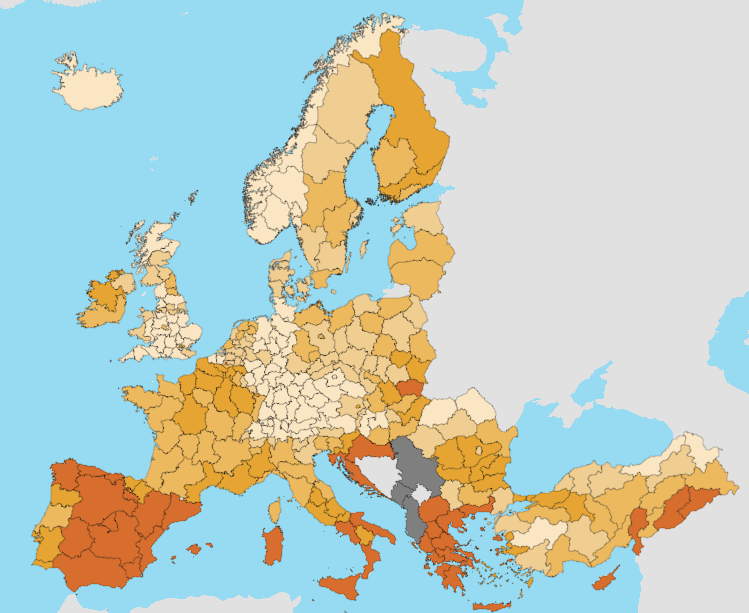
\includegraphics[width=0.99\textwidth]{../../figures/eurostat}
		\column{.5\textwidth}
		\pause
	\begin{itemize}[<+->]
		\item Conflicting findings in existing literature
		\begin{block}{}
			>>(...) the local economy \alert{has an impact} on presidential election outcomes (...)<< (Lenz \& Healy, forthcoming)
		\end{block}
		\begin{block}{}
			>>(...) local economic conditions related to the housing market \alert{do not appear to play an important role} in U.S. election results (...)<< (Hall et al., 2017) \pause
		\end{block}
	\end{itemize}
\end{columns}

\end{frame}

\begin{frame}
\begin{itemize}[<+->]
	\item Our argument: conditional on \textit{contextual priming} from local econ activity	
	\item $\rightarrow$ citizens more responsive when local econ activity is salient
	\item focus on housing market (empirically important, high-quality local data)
	\begin{exampleblock}{}
		>>\textit{H1 (Local economic conditions hypothesis)}: When local house prices rise, individuals are more likely to support the incumbent government.<<
	\end{exampleblock}
	\begin{exampleblock}{}
		>>\textit{H2 (Contextual priming hypothesis)}: The association between changes in local house prices and support for the incumbent government is stronger when individuals are more exposed to local housing market activity.<<
	\end{exampleblock}

\end{itemize}

\end{frame}

\section{Data}

\subsection{Empirical setting}
\begin{frame}
Denmark ca. 2002 - 2015.\pause

\begin{columns}

\column{.4\linewidth}	

\begin{itemize}[<+->]
	\item experienced very volatile housing bubble
	\item detailed data from the public registries on local housing markets 
	\item link the housing market data to voting behavior in two different data sets:
	\begin{itemize}[<+->]
		\item precinct-level election returns
		\item two-wave panel survey of reported voting
	\end{itemize}
\end{itemize}

\column{.6\linewidth}	

	\begin{figure}[htbp!]
	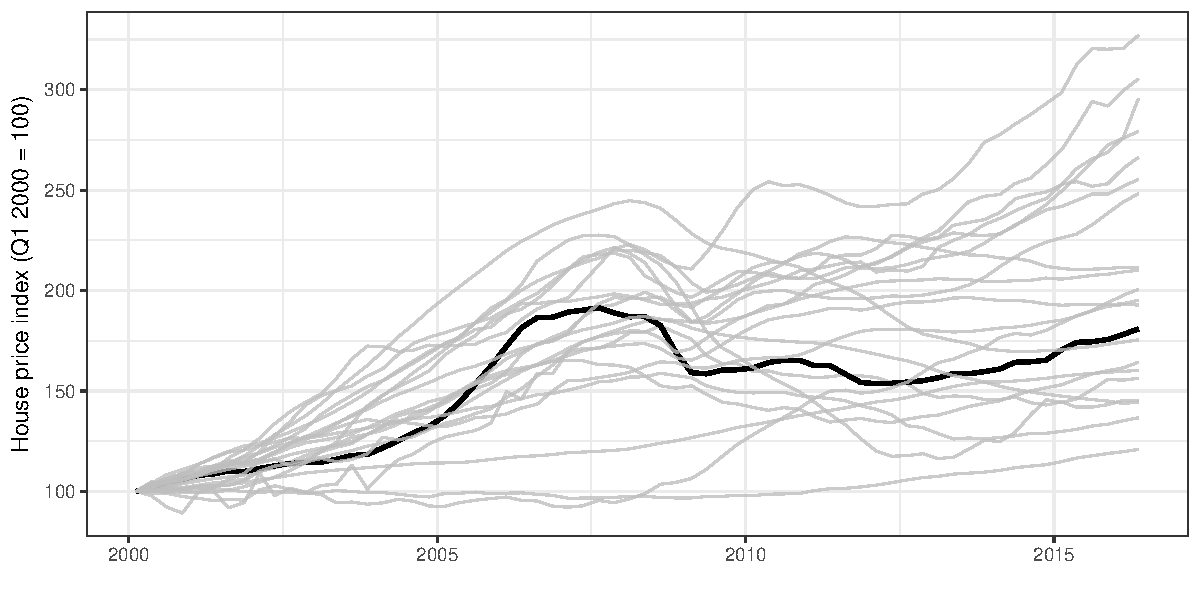
\includegraphics[width=0.9\textwidth]{../../figures/timeplot}
	\centering
	\caption{Trends in real house prices. Source: The International House Price Database.}\label{hpd}
\end{figure}

\end{columns}


\end{frame}

\subsection{Precinct-level data}

\begin{frame}
DV: support for gov't parties at precincts across elections in '05, '07, '11, '15. \\
$\rightsquigarrow$  smallest unit at which election outcomes are observed ($3,000$ voters on average) \\

\vspace{0.2in} \pause
IV: year-over-year change in the price of real-estate sold in precinct's zip code \\

\vspace{0.2in} \pause
salience measure: logged number of trades in precinct's zip code in most recent quarter

%$\rightsquigarrow$ Data from the Danish Mortgage Federation. 
\pause

\vspace{0.2in}

we link precincts to zip-codes by identifying the zip code of the precinct's polling place.

$\rightsquigarrow$  we also have information on unemployment and median income in each zip-code.



\end{frame}

\begin{frame} 
\begin{center}	
\huge{ \noindent $govt_{it}=$  $\Delta price_{it} $ \only<1>{$+ \epsilon_{it}$} \pause $+ \gamma_t$ \only<2>{$+ \epsilon_{it}$} \pause $+ \pi_i$ \only<3>{$+ \epsilon_{it}$} \pause  $+ econ \beta$ \only<4->{$+ \epsilon_{it}$} \pause

\vspace{0.2in}
\noindent $govt_{it-1}=$  $\Delta price_{it} $ $+ \gamma_t$ $+ \pi_i$  $+ econ \beta$ $+ \epsilon_{it}$
}
\end{center}
\end{frame}



\begin{frame} \centering
\foreach \n in {1,2,3,4,5,6}{

\includegraphics<\n>[width=0.8\textwidth]{../../figures/lagd\n.eps}
}
\end{frame}




\subsection{Individual-level data}

%\begin{frame}
%Use a two-wave panel survey of Danish citizens; interviewed in the aughts, '11. \pause
%
%
%$\rightsquigarrow$ Link these respondents to the national registers.
%
%\vspace{0.1in} \pause
%
%Why use this data as well?
%\begin{itemize} \pause
%\item Replication (/methodological triangulation). \pause
%\item Explore individual level moderators to get at mechanism. \pause
%\item Allows us to define context in flexible ways (cf. MAUP).
%\end{itemize}
%\end{frame}

\begin{frame}
DV: self-reported for gov't parties in most recent election \\
\vspace{0.2in} \pause
IV: year-over-year change in the price of real-estate sold in (various measures of)  respondent's context \\
\vspace{0.2in} \pause
salience measure: individuals' temporal proximity to moving, before or after survey \\
\vspace{0.2in} \pause
we use a linear regr with fixed effects to estimate the effect of local housing prices. \\ \pause
$\rightsquigarrow$ controls: unemployment, income (personal, context) \\ \pause
$\rightsquigarrow$ use LPM as a link function. 
\end{frame}

\begin{frame} 
\centering

\foreach \n in {1,2,3,4,5,6}{\noindent \begin{adjustbox}{max width=0.5\textwidth} \only<\n>{\input{../../figures/illustrate\n.txt} } \end{adjustbox}}	 
\end{frame}


\section{Results}
\subsection{}

\subsection{Precint-level data}

\begin{frame}
H1:
\begin{figure}[htbp!]
	\includegraphics[width=0.9\textwidth]{../../figures/lagdv.eps}
	\centering
	\caption{Effects of Housing Prices on support for governing party at the present election (t) and the last election (t-1) with 90  and 95 pct. Confidence Intervals}\label{placebo}
\end{figure}
\end{frame}

\begin{frame}
H2: \\
\centering
\begin{figure}[htbp!]
	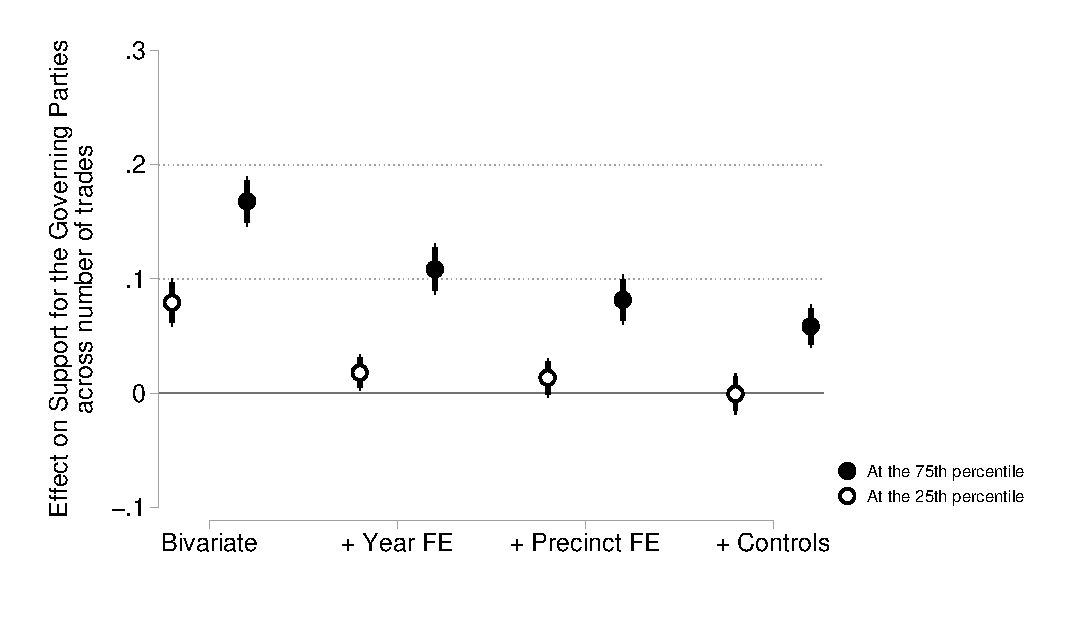
\includegraphics[width=0.9\textwidth]{../../figures/localactivity.eps}
\end{figure}
\end{frame}

\subsection{Individual-level data}

\begin{frame}
H1: \\ \centering
\foreach \n in {1,2,3,4,5,6,7}{
	
	\includegraphics<\n>[width=0.8\textwidth]{../../figures/comparison\n.eps}
}
%Not significant
\end{frame}

\begin{frame}
H2: \\ 
\centering
\begin{figure}[htbp!]
	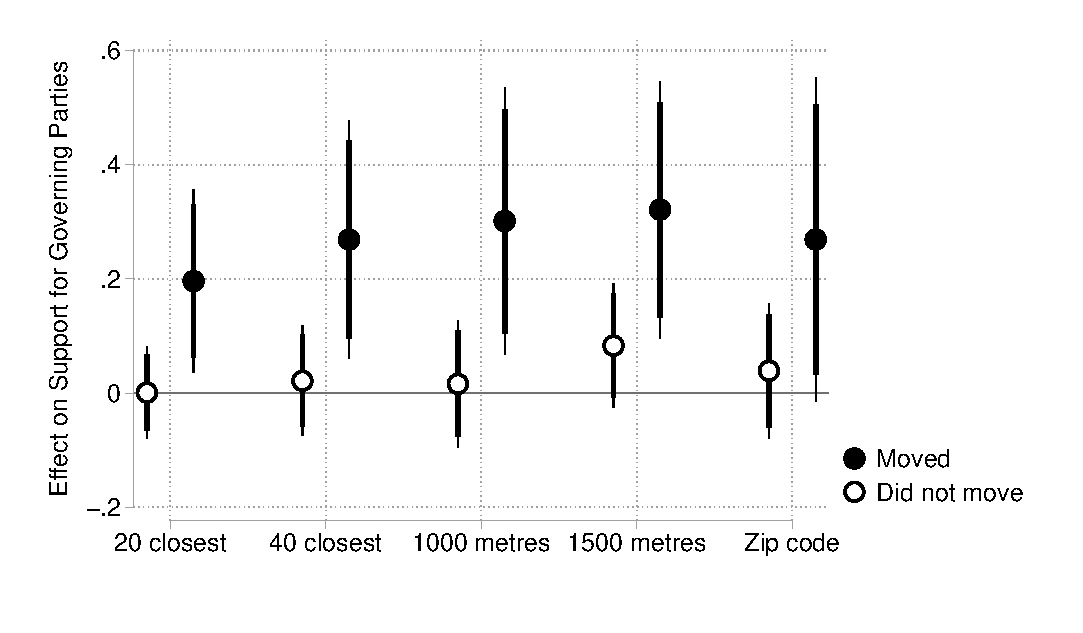
\includegraphics[width=0.9\textwidth]{../../figures/moving.eps}
\end{figure}
\end{frame}



\section{Conclusion}
\subsection{}
\begin{frame}
local economic conditions (housing prices) do drive incumbent support \\ \pause
$\rightsquigarrow$ effect stronger where/when individuals engage with the local housing market \pause

\vspace{0.2in}
suggests that local economy matters \pause
\begin{itemize}[<+->]
\item individuals make inferences about incumbents based on how local community is doing.
\item pol's need to worry about `geography of grievances'.
\end{itemize}

\vspace{0.2in} \pause
housing markets (also) matter politically \\ \pause
$\rightsquigarrow$ voters adapt to changing economies, focus on new parts of the economy
\end{frame}

\begin{frame}
\centering
Thanks for your time!
\end{frame}

\appendix

\begin{frame} \centering
\foreach \n in {1,2,3,4,5,6,7}{
	
	\includegraphics<\n>[width=1\textwidth]{../../figures/moderator\n.eps}
}

%Not significant
\end{frame}
	
\end{document}
	
